\documentclass[a4paper,11pt]{article}

\author{wilricknl}
\title{3D Math Primer - Notes}

\usepackage{amsmath}
\usepackage{amssymb}
\usepackage{float}
\usepackage{graphicx}
\graphicspath{ {./images/} }
\usepackage{tikz}
\usetikzlibrary{arrows.meta}
\usepackage{url}

% clickable URLs
\usepackage{color}
\usepackage{hyperref}
\hypersetup{
    colorlinks,
    citecolor=black,
    filecolor=black,
    linkcolor=black,
    urlcolor=black
}

\begin{document}

\maketitle

\newpage
\tableofcontents

\newpage
\section{Introduction}

This document is a reference of the things most interesting to me from 3D math primer. This document is by no means a tutorial, so whenever something is unclear: step up your game and figure it out.

\subsection{Conventions}

\begin{itemize}
\item A left handed coordinate space is assumed unless specified otherwise.
\item \textit{Scalar} variables are represented by lowercase Roman or Greek letters in italics: $a$, $b$, $x$, $y$, $z$, $\theta$,
  $\alpha$, $\omega$, $\gamma$.
\item
  \textit{Vector} variables of any dimension are represented by lowercase
  letters in boldface: $\mathbf{a}$, $\mathbf{b}$, $\mathbf{u}$, $\mathbf{v}$, $\mathbf{q}$, $\mathbf{r}$.
\item \textit{Matrix} variables are represented using uppercase letters in
  boldface: $\mathbf{A}$, $\mathbf{B}$, $\mathbf{M}$, $\mathbf{R}$.
 \item \textit{Quaternion} variables are represented by lowercase letters in boldface: $\textbf{q}$. The difference between quaternions and vectors will be clear by the context.
\end{itemize}

\subsection{Math notation}

\begin{itemize}
	\item \textit{Interval notation}; often times a range of numbers is required. For this we use interval notation. I always forget about it, so I guess it's useful to write it all down:
	\begin{itemize}
		\item \textit{Open} interval: $(0,1)$ denotes all points $0 < x < 1$.
		\item \textit{Closed} interval: $[0,\pi]$ denotes all points $0 \leq x \leq \pi$.
		\item \textit{Mixed} intervals: $(-90^\circ, 90^\circ]$ denotes the points $90^\circ < x \leq 90^\circ$.
	\end{itemize}
\end{itemize}


% Chapter 1 of the book
\newpage
\section{Cartesian Coordinate Systems}

\subsection{Coordinate system handedness}

In 3D space there are two types of coordinate systems: the so-called left and right handed coordinate systems. The way to recreate these systems is to make your index fingers pointer up, then your thumbs should point to each other, while your third finger points away from you. Just like in algebra class your index finger represents the $y$-axis, your thumbs the $x$-axis, while your third finger represents the $z$-axis.

\begin{figure}[H]
\centering
    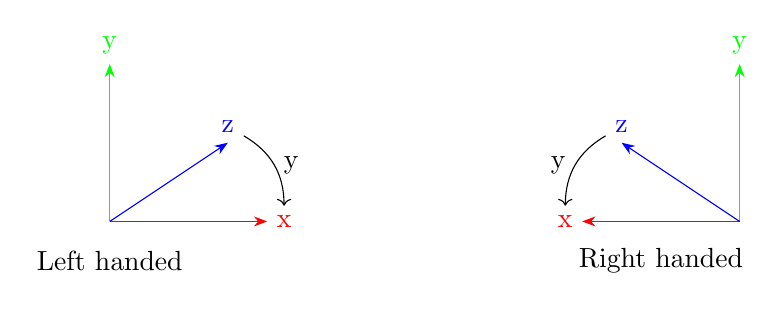
\begin{tikzpicture}
		\draw [red,-{Stealth}] (-4,0)--(-2,0) node[right] (xleft) {x};        
		\draw [green,-{Stealth}] (-4,0)--(-4,2) node[above]{y};       
		\draw [blue,-{Stealth}] (-4,0)--(-2.5,1) node[above] (zleft) {z};  
		\draw[->] (zleft) to[bend left] node [right] {y} (xleft);
		\node at (-4,-0.5) {Left handed};      
        
		\draw [red,{Stealth}-] (2,0) node[left] (xright) {x} -- (4,0);        
		\draw [green,-{Stealth}] (4,0)--(4,2) node[above]{y};       
		\draw [blue,-{Stealth}] (4,0)--(2.5,1) node[above] (zright) {z};
		\draw[->] (zright) to[bend right] node [left] {y} (xright);  
		\node at (3,-0.5) {Right handed};
		                
    \end{tikzpicture}
\caption{Coordinate system handedness}
\label{fig:coordinate-system-handedness}
\end{figure}

Rotation in a left handed in a left handed system is clock wise, while positive in a right handed system is counter clock wise. In figure  \ref{fig:coordinate-system-handedness} the $y$-rotation of both  coordinate systems is visualized with the black arrow. A trick to remember is to put your thumb up and see how your fingers curl around your palm.

\begin{quote}
\emph{Within these notes I follow the book and use the left handed system as visualized in figure \ref{fig:coordinate-system-handedness}.}
\end{quote}

\subsection{Trigonometry}

\subsubsection{Degrees and radians}

\[
\begin{array}{rll}
{1\ {rad} =} & {\left( 180/\pi \right)^{o}} & {\approx 57.29578^{o},} \\
{1^{o} =} & {\left( \pi/180 \right)\ {rad}} & {\approx 0.01745329\ {rad}.} \\
\end{array}
\]


\subsubsection{Functions}

\begin{align*}
\cos\theta &=x, &\sin\theta &=y, \\
\sec\theta &=\frac{1}{\cos\theta}, &\tan\theta &=\frac{\sin\theta}{\cos\theta}, \\
\csc\theta &=\frac{1}{\sin\theta}, &\cot\theta &=\frac{1}{\tan\theta}=\frac{\cos\theta}{\sin\theta}.
\end{align*}

\subsubsection{SOH CAH TOA}

The primary function are defined by the ratios of a \emph{right} triangle. Note that when the angle is obtuse, i.e. $90^\circ < \theta < 180^\circ$, the ratios do not work.

\begin{figure}[H]
\centering
    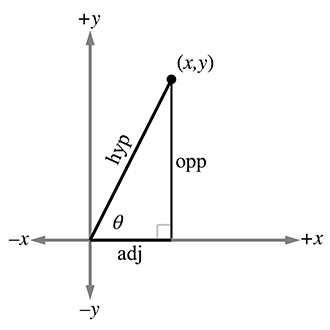
\includegraphics{01_sohcahtoa}
\caption{SOH CAH TOA visualisation}
\label{fig:soh-cah-toa-visualization}
\end{figure}

\[\begin{matrix}
{\cos\theta} & {= \frac{\mathit{a}\mathit{d}\mathit{j}}{\mathit{h}\mathit{y}\mathit{p}},} & {\sin\theta} & {= \frac{\mathit{o}\mathit{p}\mathit{p}}{\mathit{h}\mathit{y}\mathit{p}},} & {\tan\theta} & {= \frac{\mathit{o}\mathit{p}\mathit{p}}{\mathit{a}\mathit{d}\mathit{j}},} \\
 & & & & & \\
{\sec\theta} & {= \frac{\mathit{h}\mathit{y}\mathit{p}}{\mathit{a}\mathit{d}\mathit{j}},} & {\csc\theta} & {= \frac{\mathit{h}\mathit{y}\mathit{p}}{\mathit{o}\mathit{p}\mathit{p}},} & {\cot\theta} & {= \frac{\mathit{a}\mathit{d}\mathit{j}}{\mathit{o}\mathit{p}\mathit{p}}.} \\
\end{matrix}\]

The general definitions are defined as follows:
\begin{figure}[H]
\centering
    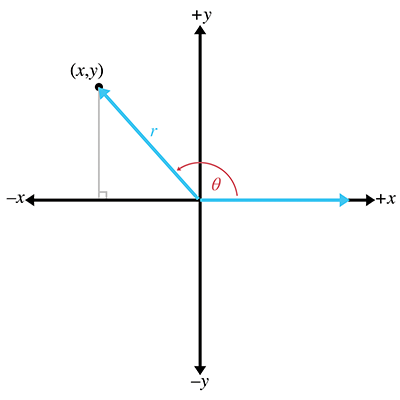
\includegraphics{01_general_trigonometry_definitions}
\caption{General trigonometry definitions}
\label{fig:general-trigonometry-definitions}
\end{figure}

\[\begin{matrix}
{\cos\theta} & {= x/r,} & {\sin\theta} & {= y/r,} & {\tan\theta} & {= y/x,} \\
 & & & & & \\
{\sec\theta} & {= r/x,} & {\csc\theta} & {= r/y,} & {\cot\theta} & {= x/y.} \\
\end{matrix}\]

\subsubsection{Identities}

\[
\begin{array}{rlrlrl}
{\sin( - \theta) =} & {- \sin\theta,} & {\cos( - \theta) =} & {\cos\theta,} & {\tan( - \theta) =} & {- \tan\theta,} \\
{\sin\left( \frac{\pi}{2} - \theta \right) =} & {\cos\theta,} & {\cos\left( \frac{\pi}{2} - \theta \right) =} & {\sin\theta,} & {\tan\left( \frac{\pi}{2} - \theta \right) =} & {\cot\theta.}
\end{array}
\]

\subsubsection{Common values}

\(\begin{matrix}
{\theta^{o}} & {\theta\ {rad}} & {\cos\theta} & {\sin\theta} & {\tan\theta} & {\sec\theta} & {\csc\theta} & {\cot\theta} \\
0 & 0 & 1 & 0 & 0 & 1 & {undef} & {undef} \\
30 & {\frac{\pi}{6} \approx 0.5236} & \frac{\sqrt{3}}{2} & \frac{1}{2} & \frac{\sqrt{3}}{3} & \frac{2\sqrt{3}}{3} & 2 & \sqrt{3} \\
45 & {\frac{\pi}{4} \approx 0.7854} & \frac{\sqrt{2}}{2} & \frac{\sqrt{2}}{2} & 1 & \sqrt{2} & \sqrt{2} & 1 \\
60 & {\frac{\pi}{3} \approx 1.0472} & \frac{1}{2} & \frac{\sqrt{3}}{2} & \sqrt{3} & 2 & \frac{2\sqrt{3}}{3} & \frac{\sqrt{3}}{3} \\
90 & {\frac{\pi}{2} \approx 1.5708} & 0 & 1 & {undef} & {undef} & 1 & 0 \\
120 & {\frac{2\pi}{3} \approx 2.0944} & {- \frac{1}{2}} & \frac{\sqrt{3}}{2} & {- \sqrt{3}} & {- 2} & \frac{2\sqrt{3}}{3} & {- \frac{\sqrt{3}}{3}} \\
135 & {\frac{3\pi}{4} \approx 2.3562} & {- \frac{\sqrt{2}}{2}} & \frac{\sqrt{2}}{2} & {- 1} & {- \sqrt{2}} & \sqrt{2} & {- 1} \\
150 & {\frac{5\pi}{6} \approx 2.6180} & {- \frac{\sqrt{3}}{2}} & \frac{1}{2} & {- \frac{\sqrt{3}}{3}} & {- \frac{2\sqrt{3}}{3}} & 2 & {- \sqrt{3}} \\
180 & {\pi \approx 3.1416} & {- 1} & 0 & 0 & {- 1} & {undef} & {undef} \\
210 & {\frac{7\pi}{6} \approx 3.6652} & {- \frac{\sqrt{3}}{2}} & {- \frac{1}{2}} & \frac{\sqrt{3}}{3} & {- \frac{2\sqrt{3}}{3}} & {- 2} & {- \sqrt{3}} \\
225 & {\frac{5\pi}{4} \approx 3.9270} & {- \frac{\sqrt{2}}{2}} & {- \frac{\sqrt{2}}{2}} & 1 & {- \sqrt{2}} & {- \sqrt{2}} & {- 1} \\
240 & {\frac{4\pi}{3} \approx 4.1888} & {- \frac{1}{2}} & {- \frac{\sqrt{3}}{2}} & \sqrt{3} & {- 2} & {- \frac{2\sqrt{3}}{3}} & {- \frac{\sqrt{3}}{3}} \\
270 & {\frac{3\pi}{2} \approx 4.7124} & 0 & {- 1} & {undef} & {undef} & {- 1} & 0 \\
300 & {\frac{5\pi}{3} \approx 5.2360} & \frac{1}{2} & {- \frac{\sqrt{3}}{2}} & {- \sqrt{3}} & 2 & {- \frac{2\sqrt{3}}{3}} & {- \frac{\sqrt{3}}{3}} \\
315 & {\frac{7\pi}{4} \approx 5.4978} & \frac{\sqrt{2}}{2} & {- \frac{\sqrt{2}}{2}} & {- 1} & \sqrt{2} & {- \sqrt{2}} & {- 1} \\
330 & {\frac{11\pi}{6} \approx 5.7596} & \frac{\sqrt{3}}{2} & {- \frac{1}{2}} & {- \frac{\sqrt{3}}{3}} & \frac{2\sqrt{3}}{3} & {- 2} & {- \sqrt{3}} \\
360 & {2\pi \approx 6.2832} & 1 & 0 & 0 & 1 & {undef} & {undef} \\
\end{matrix}\)

\subsubsection{Sum and difference identities}

\[\begin{matrix}
{\sin(a + b)} & {= \sin a\cos b + \cos a\sin b,} \\
{\sin(a - b)} & {= \sin a\cos b - \cos a\sin b,} \\
{\cos(a + b)} & {= \cos a\cos b - \sin a\sin b,} \\
{\cos(a - b)} & {= \cos a\cos b + \sin a\sin b,} \\
{\tan(a + b)} & {= \frac{\tan a + \tan b}{1 - \tan a\tan b},} \\
{\tan(a - b)} & {= \frac{\tan a - \tan b}{1 + \tan a\tan b}.} \\
\end{matrix}\]

\subsubsection{Pythagorean identities}

\[\begin{matrix}
{\sin^{2}\theta + \cos^{2}\theta} & {= 1,} & {1 + \tan^{2}\theta} & {= \sec^{2}\theta,} & {1 + \cot^{2}\theta} & {= \csc^{2}\theta.} \\
\end{matrix}\]

\subsubsection{Double angle identities}

\[\begin{matrix}
{\sin 2\theta} & {= 2\sin\theta\cos\theta,} \\
{\cos 2\theta} & {= \cos^{2}\theta - \sin^{2}\theta = 2\cos^{2}\theta - 1 = 1 - 2\sin^{2}\theta,} \\
{\tan 2\theta} & {= \frac{2\tan\theta}{1 - \tan^{2}\theta}.} \\
\end{matrix}\]

\subsubsection{Law of sines and cosines}

\begin{figure}[H]
\centering
    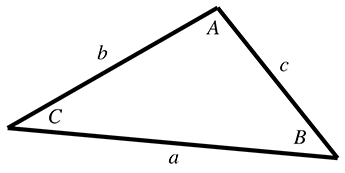
\includegraphics{01_laws}
\caption{Laws of sines and cosines}
\label{fig:laws-of-sines-and-cosines}
\end{figure}

$$\frac{\sin A}{a}=\frac{\sin B}{b}=\frac{\sin C}{c}$$

\begin{align*}
a^2 &= b^2 + c^2 - 2bc\cos A, \\
b^2 &= a^2 + c^2 - 2ac\cos B, \\
c^2 &= a^2 + b^2 - 2ab\cos C.
\end{align*}


% Chapter 2 of the book
\newpage
\section{Vectors}

Vectors are basically an array of numbers which can be used to do cool calculations. We differentiate between two types of vectors: \textit{row} and \textit{column} vectors. The difference between them becomes especially important when multiplying matrices with vectors. Row vectors require post-multiplication, while column vectors require pre-multiplication.

$$
\begin{array}{cc}
\textbf{a} = \begin{bmatrix}
1 & 2 & 3
\end{bmatrix},
&
\textbf{b} = \begin{bmatrix}
4 \\ 5 \\ 6
\end{bmatrix}
\end{array}
$$

\subsection{Magnitude}

The \textit{magnitude} describes the length of the vectors. The length may be any non-negative length. The \textit{direction} of a vectors describes which the vector is pointing. The magnitude can be calculated by taking taking the square root of the summation of the squares of all scalars in the vector. A three dimensional example:

$$\|\textbf{v}\|=\sqrt{{v_x}^2+{v_y}^2+{v_z}^2}$$

\subsection{Unit vector}

A unit vector can be calculated by dividing the vector by its magnitude.

$$\hat{\textbf{v}}=\frac{\textbf{v}}{\|\textbf{v}\|}$$

\subsection{Distance between two vectors}

The distance between two vectors can be calculated by subtracting the two vectors from each other, then calculating the magnitude.

$$\|b-a\|=\sqrt{(b_x-a_x)^2+(b_y-a_y)^2+(b_z-a_z)^2}$$

\subsection{Dot product}

The dot product is the first way of multiplying vectors together. The other one being the cross product, which is the topic of the next section. The way the dot product works is rather simple, but it is mostly the interpretation of its power that makes it a bit more difficult to wrap your head around.

$$\textbf{a}\cdot\textbf{b}=a_xb_x+a_yb_y+a_zb_z$$

$$
\begin{bmatrix}
1 \\ 2 \\ 3
\end{bmatrix} \cdot
\begin{bmatrix}
4 \\ 5 \\ 6
\end{bmatrix}=(1)(4)+(2)(5)+(3)(6)=4+10+18=32
$$

It is simply matching the right scalars and adding it all together, but what does this actually mean?

\subsubsection{Parallel and perpendicular vector}

Using the dot product we can project one vector on another vector. Take the dot product $\hat{\textbf{a}}\cdot\textbf{b}$. By taking the dot product we know how much of $\textbf{b}$ goes parallel to $\textbf{a}$, because $\textbf{a}$ is a unit vector. The dot product returns a scalar, so multiplying this scalar by $\hat{\textbf{a}}$ we calculated $\textbf{b}_\|$, that is the part of $\textbf{b}$ parallel to $\textbf{a}$. The part of $\textbf{b}$ perpendicular to $\textbf{a}$ can be calculated by $\textbf{b}-\textbf{b}_\|=\textbf{b}_\perp$. Putting it all together:

$$\textbf{b}_\|=(\hat{\textbf{a}}\cdot\textbf{b})\hat{\textbf{a}}$$
$$\textbf{b}_\perp=\textbf{b}-\textbf{b}_\|=\textbf{b}-(\hat{\textbf{a}}\cdot\textbf{b})\hat{\textbf{a}}$$
$$\textbf{b}=\textbf{b}_\|+\textbf{b}_\perp$$

\begin{figure}[H]
\centering
    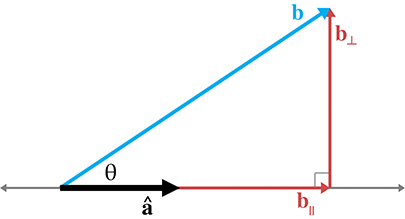
\includegraphics{02_vector_projection}
\caption{Vector projection}
\label{fig:vector-projection}
\end{figure}

\subsubsection{Visibility}

Using the sign of the dot product we can determine where two vectors are in relation to each other.

\begin{figure}[H]
\centering
    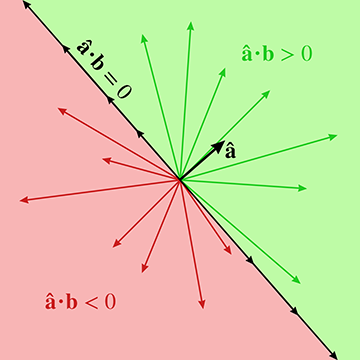
\includegraphics{02_dot_signs}
\caption{Dot product signs}
\label{fig:dot-product-signs}
\end{figure}

\begin{itemize}
	\item A positive dot product means $\textbf{b}$ is in front of $\textbf{a}$.
	\item A negative dot product means $\textbf{b}$ is behind $\textbf{a}$.
	\item A dot product with value 0 means that $\textbf{b}$ is exactly to the left or right of $\textbf{a}$.
\end{itemize}

Some nice calculations and practice with this concept can be found in exercises 20 and 21 of chapter 2. These exercises take distance and field of view into account.

\subsubsection{Cosine angle between two vectors}

The final interpretation is to calculate the angle between two vectors using the dot product. The first thing to remember is that $\cos\theta=\frac{\text{adjecent}}{\text{hypotenuse}}$. With the dot product we calculate how much one vector projects on to the other, thus calculating the adjacent value and creating a right triangle as shown in the image below. Assuming unit vectors as shown in the image we derive $\cos\theta=\frac{\text{adjecent}}{\text{hypotenuse}}=\frac{\hat{\textbf{a}}\cdot\hat{\textbf{b}}}{1}=\hat{\textbf{a}}\cdot\hat{\textbf{b}}$. The general formula that does not assume unit vectors is therefore:

$$\cos\theta=\frac{\hat{\textbf{a}}\cdot\hat{\textbf{b}}}{\|\textbf{a}\|\|\textbf{b}\|}$$

Then to get the actual angle:

$$\theta=\arccos\left(\frac{\hat{\textbf{a}}\cdot\hat{\textbf{b}}}{\|\textbf{a}\|\|\textbf{b}\|}\right)$$

\begin{figure}[H]
\centering
    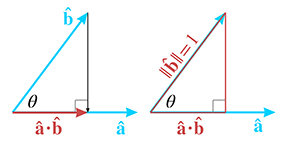
\includegraphics{02_dot_angle}
\caption{Dot product angle}
\label{fig:dot-product-angle}
\end{figure}

Now we can put all this angle calculation into perspective. Take a look at the following table which shows exactly why we were able to use the sign of the dot product to determine if if two vectors are visible with respect to each other.

\begin{table}[H]
\centering
\begin{tabular}{|l|l|l|l|l|}
\hline
$\textbf{a}\cdot\textbf{b}$ & $\theta$ & \textbf{Angle is} & $\textbf{a}$ \textbf{and} $\textbf{b}$ \textbf{are}  \\ \hline
$>0$ & $0^\circ \leq \theta < 90^\circ$ & acute & pointing mostly in the same direction. \\ \hline
$0$ & $\theta=90^\circ$ & right & perpendicular \\ \hline
$<0$ & $90^\circ < \theta \leq 180^\circ$ & obtuse & pointing mostly in the same direction \\ \hline
\end{tabular}
\caption{Dot product angles}
\label{tab:dot-product-angles}
\end{table}

\subsubsection{Magnitude}

A nice thing to realize is that taking the dot product of a vector itself results into the square of its magnitude: $\textbf{v}\cdot\textbf{v}=\|\textbf{v}\|^2$, so $\|\textbf{v}\|=\sqrt{\textbf{v}\cdot\textbf{v}}$.

\subsection{Cross product}

The cross product is slightly more difficult to calculate and does not exist for two dimensional vectors. Unlike the dot product the cross product does not return a scalar, but a vector instead. The general formula is:

$$
\textbf{a}\times\textbf{b}=
\begin{bmatrix}
a_x \\ a_y \\ a_z
\end{bmatrix}\times
\begin{bmatrix}
b_x \\ b_y \\ b_z
\end{bmatrix}=
\begin{bmatrix}
a_yb_z - a_zb_y \\ a_zb_x - a_xb_z \\ a_xb_y - a_yb_x
\end{bmatrix}
$$

\subsubsection{Perpendicular vector}

The geometric interpretation of the cross product is to visualize a third vector perpendicular to the vectors which were used to calculate the cross product. This is for example used to calculate surface normals, but more about that later.

\begin{figure}[H]
\centering
    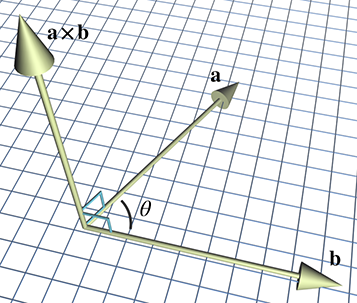
\includegraphics{02_cross_product}
\caption{Cross product}
\label{fig:cross-product}
\end{figure}

\subsubsection{Sine angle between two vectors}

The cross product has a similar usage as the dot product to calculate an angle between two vectors. In this case it is possible to calculate the sine between two vectors as follows: $\sin\theta=\frac{\|\textbf{a}\times\textbf{b}\|}{\|\textbf{a}\|\|\textbf{b}\|}$.


% Chapter 3 of the book
\newpage
\section{Multiple coordinate spaces}

Coordinate spaces are all over the place. In robotics a point cloud is defined in the space of its sensor. To make actual use of this data we transform the point cloud to be in the space of the robot itself. It is a requirement to be able to think in different coordinate spaces in order to do any serious work. Let's quickly take a look at some common coordinate spaces and how to transform between one coordinate space and another.

\subsection{Common coordinate spaces}

\subsubsection{Object space}

The object space describes vertices of some object to a shared origin. When artists create some model, e.g. a tank, they start modelling the various meshes around an origin within a modelling program like Blender. All the vertices of the various meshes of the model are saved to some file which can be loaded by a game engine.

\subsubsection{World space}

Any interesting game consists of various models each described in their own object space. However, to create a nice world every model gets placed at some world coordinate relative from each other. To properly display the created world all coordinates need to be transformed to this shared world.

\subsubsection{Upright space}

Upright space is a step between object and world space. In upright space the rotation of the world space is already applied. To go from upright space to world space only requires some translation. This space is not always used in tutorials or books, but it is a nice step to make it easier to reason about a switch between coordinate spaces.

\subsubsection{Camera space}

Camera space is the object space associated with the viewpoint used for rendering. The camera space determines which parts of the world are visible.

\subsection{Object space to world space}

Let's take a brief look at an example of transforming a simple pyramid from object space to some world space. First, of all let's define the vertices of the pyramid.

\begin{itemize}
	\item Top: $\begin{bmatrix}
		0 & 2 & 0
	\end{bmatrix}^\intercal$
	\item Front left: $\begin{bmatrix}
		-2 & 0 & -2
	\end{bmatrix}^\intercal$
	\item Front right: $\begin{bmatrix}
		2 & 0 & -2
	\end{bmatrix}^\intercal$
	\item Back left: $\begin{bmatrix}
		-2 & 0 & 2
	\end{bmatrix}^\intercal$
	\item Back right: $\begin{bmatrix}
		2 & 0 & 2
	\end{bmatrix}^\intercal$
\end{itemize}

Furthermore, we know that the world position to be $\begin{bmatrix}2 & 0 & 3\end{bmatrix}^\intercal$, the used coordinate system is left handed and the pyramid is rotated $45^\circ$. With this information we can also state the basis vectors relative to the world space.

\begin{itemize}
	\item Position: $\begin{bmatrix}2 & 0 & 3\end{bmatrix}^\intercal$
	\item $\textbf{p}=\begin{bmatrix}0.707 & 0 & 0.707\end{bmatrix}^\intercal$
	\item $\textbf{q}=\begin{bmatrix}0 & 1 & 0\end{bmatrix}^\intercal$
	\item $\textbf{r}=\begin{bmatrix}0.707 & 0 & -0.707\end{bmatrix}^\intercal$
\end{itemize}

$\textbf{p}$, $\textbf{q}$ and $\textbf{r}$ is a common notation to denote the basis vectors. Basis vectors specify how to interpret coordinates within its space. Good basis vector are orthonormal, that is all vectors are perpendicular to each other and of unit length. Read the book for the exact reasons why. Yup, I choose the easy way out. Now onto the fun part: converting object coordinates to world space!

To transform the vertices of the pyramid to world space we need to apply its basis vectors. Basis vector can contain various transformation like scaling, reflection and rotation. More about these in the chapter about matrices. In this case we only store the rotation relative to the world space. Once the basis vectors are applied all vertices are defined in terms of \textit{upright space}. All that is left to do is to translate all vertices by the position the pyramid is assigned within world space. After this final step all vertices are defined in terms of world space. Note that upright space is not necessary to define explicitly, but it makes it easier to reason about the transformation.

\subsubsection{Transforming a single vertex}

As an example let's transform the front left vertex ($\begin{bmatrix}
		-2 & 0 & -2
	\end{bmatrix}^\intercal$) from object space to world space. Thus we need to apply the basis vectors to the vertex:

$$\textbf{u}=-2\begin{bmatrix}0.707 \\ 0 \\ 0.707\end{bmatrix}+0+-2\begin{bmatrix}0.707 \\ 0 \\ -0.707\end{bmatrix}=\begin{bmatrix}-2.828 \\ 0 \\ 0\end{bmatrix}$$

As stated in the previous chapter the dot product is able to determine how much of a vector goes into a specific direction. This is exactly why we apply the basis vectors against the $x$, $y$, and $z$ coordinate. Now that the axes are aligned there is one final step remaining: we have to add the world position the the upright coordinate:

$$\textbf{w}=\begin{bmatrix}-2.828 \\ 0 \\ 0\end{bmatrix}+\begin{bmatrix}2 \\ 0 \\ 3\end{bmatrix}=\begin{bmatrix}-0.828 \\ 0 \\ 3\end{bmatrix}$$

\subsubsection{Transforming the pyramid}

Let's visualize the pyramid transformation to get a better feel for these coordinate spaces. The values for each of the coordinates are specified in table \ref{tab:pyramid-coordinates-transformation}. In figure \ref{fig:pyramid-object-space} we show the pyramid in its own object space. We specified that we want to rotate our pyramid by $45^\circ$, so we expect to see a rotated pyramid in upright space (figure \ref{fig:pyramid-upright-space}). Finally, to go from upright space to world space the rotation should not just, but only a translation should be applied. This is exactly what happens in figure \ref{fig:pyramid-world-space}. So at this point mess around with the formulas a bit. Convert coordinates between the various spaces and try to understand the diagrams.

\begin{table}[H]
\centering
\begin{tabular}{|l|l|l|l|}
\hline
\textbf{Position} & \textbf{Object space} & \textbf{Upright space} & \textbf{World space} \\ \hline
Top & $\begin{bmatrix}0 & 2 & 0\end{bmatrix}^\intercal$ & $\begin{bmatrix}0 & 2 & 0\end{bmatrix}^\intercal$ & $\begin{bmatrix}2 & 2 & 3\end{bmatrix}^\intercal$ \\ \hline
Front left & $\begin{bmatrix}-2 & 0 & -2\end{bmatrix}^\intercal$ & $\begin{bmatrix}-2.828 & 0 & 0\end{bmatrix}^\intercal$ & $\begin{bmatrix}-0.828 & 0 & 3\end{bmatrix}^\intercal$ \\ \hline
Front right & $\begin{bmatrix}2 & 0 & -2\end{bmatrix}^\intercal$ & $\begin{bmatrix}0 & 0 & 2.828\end{bmatrix}^\intercal$ & $\begin{bmatrix}2 & 0 & 5.828\end{bmatrix}^\intercal$ \\ \hline
Back left & $\begin{bmatrix}-2 & 0 & 2\end{bmatrix}^\intercal$ & $\begin{bmatrix}0 & 0 & -2.828\end{bmatrix}^\intercal$ & $\begin{bmatrix}2 & 0 & 0.172\end{bmatrix}^\intercal$ \\ \hline
Back right & $\begin{bmatrix}2 & 0 & 2\end{bmatrix}^\intercal$ & $\begin{bmatrix}2.828 & 0 & 0\end{bmatrix}^\intercal$ & $\begin{bmatrix}4.828 & 0 & 3\end{bmatrix}^\intercal$ \\ \hline
\end{tabular}
\caption{Pyramid coordinates transformation}
\label{tab:pyramid-coordinates-transformation}
\end{table}

\begin{figure}[H]
\centering
    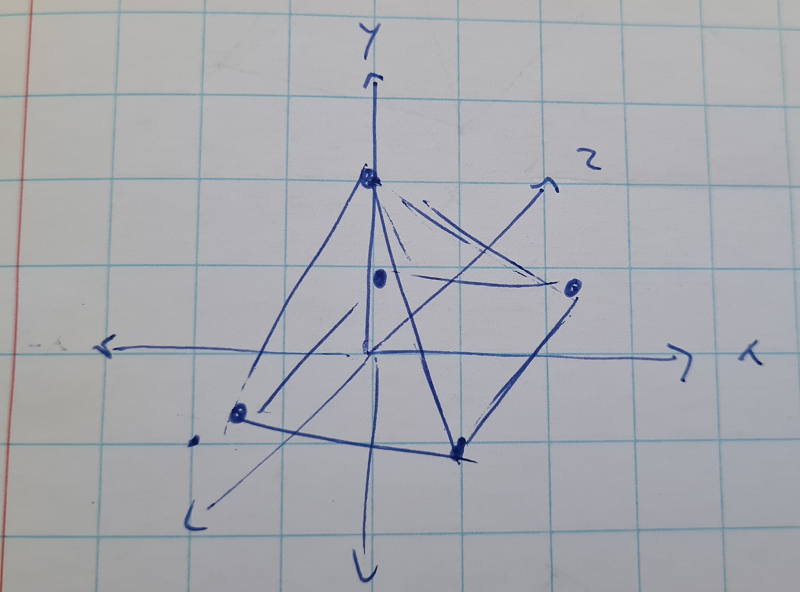
\includegraphics[scale=0.65]{03_object_space}
\caption{Pyramid in object space}
\label{fig:pyramid-object-space}
\end{figure}

\begin{figure}[H]
\centering
    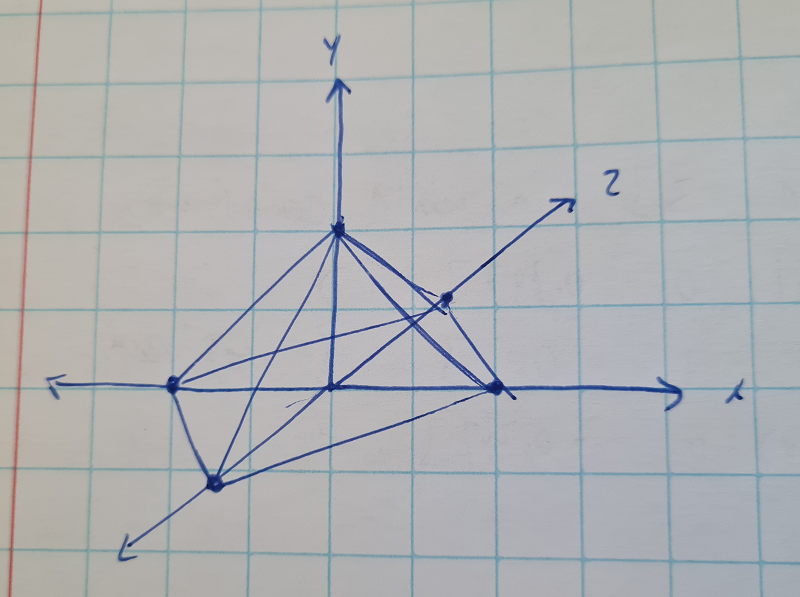
\includegraphics[scale=0.65]{03_upright_space}
\caption{Pyramid in upright space}
\label{fig:pyramid-upright-space}
\end{figure}

\begin{figure}[H]
\centering
    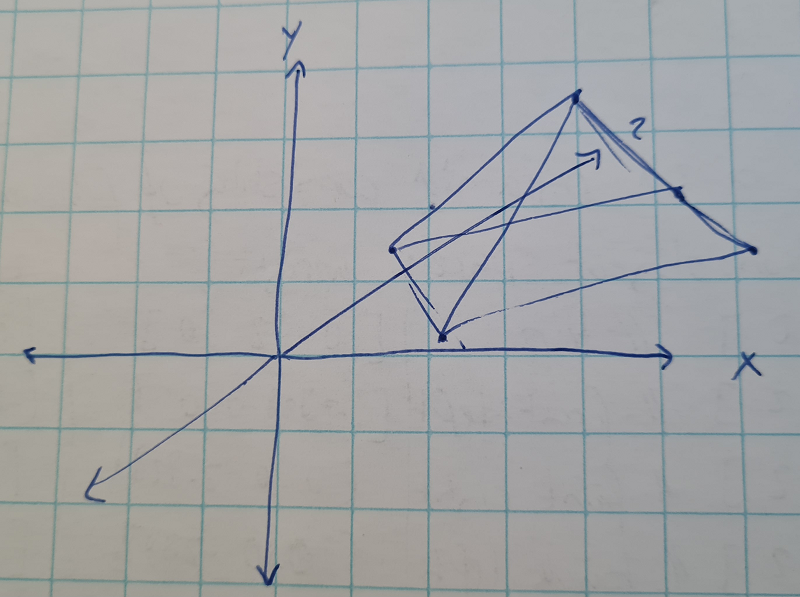
\includegraphics[scale=0.65]{03_world_space}
\caption{Pyramid in world space}
\label{fig:pyramid-world-space}
\end{figure}

\subsubsection{General formulas}

Let $\textbf{v}$ be an arbitrary vertex is object space, $\textbf{u}$ equal to $\textbf{v}$ transformed in upright space and $\textbf{w}$ equal to $\textbf{v}$ transformed in world space. Furthermore, the basis vectors $\textbf{p}$, $\textbf{q}$ and $\textbf{r}$ with world position $\textbf{o}$.

$$\textbf{u}=v_x\textbf{p}+v_y\textbf{q}+v_z\textbf{r}$$

$$\textbf{w}=\textbf{o}+\textbf{u}=\textbf{o}+v_x\textbf{p}+v_y\textbf{q}+v_z\textbf{r}$$

\subsection{Object space to world space}

To go from world space to object space we need to reverse the process described in the previous section. The formulas to achieve this are as follows:

$$\textbf{u}=\textbf{w}-\textbf{o}$$

$$\textbf{v}=\begin{bmatrix}
\textbf{u}\cdot\textbf{p} \\ \textbf{u}\cdot\textbf{q} \\ \textbf{u}\cdot\textbf{r}
\end{bmatrix}$$


% Chapter 5 of the book
\newpage	
\section{Matrices and Linear Transformations}

\subsection{Rotation matrices}\label{sec:rotation-matrices}

Make stuff spin around!

\subsubsection{Two dimensional}

\begin{figure}[H]
\centering
    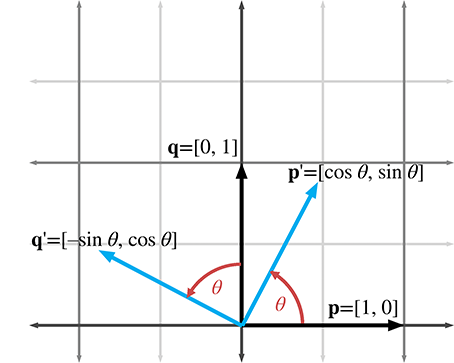
\includegraphics{05_2d_rotation}
\caption{2D rotation visualization}
\label{fig:2d-rotation-visualization}
\end{figure}

$$
\begin{matrix}
{\mathbf{R}(\theta) =
\begin{bmatrix}
{\cos\theta} & {\sin\theta} \\
{- \sin\theta} & {\cos\theta} \\
\end{bmatrix}.} \\
\end{matrix}
$$

\subsubsection{Three dimensional}

Rotation around x-axis: \\
$$
\mathbf{R}_{x}(\theta) = 
\mathbf{R}(
\begin{bmatrix}
1 & 0 & 0 
\end{bmatrix},
\theta) =
 \begin{bmatrix}
1 & 0 & 0 \\
0 & {\cos\theta} & {\sin\theta} \\
0 & {- \sin\theta} & {\cos\theta} \\
\end{bmatrix}
$$

Rotation around y-axis: \\
$$
\mathbf{R}_{y}(\theta) = 
\mathbf{R}(
\begin{bmatrix}
0 & 1 & 0 
\end{bmatrix},
\theta) = \begin{bmatrix}
{\cos\theta} & 0 & {- \sin\theta} \\
0 & 1 & 0 \\
{\sin\theta} & 0 & {\cos\theta} \\
\end{bmatrix}
$$

Rotation around z-axis: \\
$$
\mathbf{R}_{z}(\theta) =
\mathbf{R}(
\begin{bmatrix}
0 & 0 & 1
\end{bmatrix},
\theta) =
\begin{bmatrix}
{\cos\theta} & {\sin\theta} & 0 \\
{- \sin\theta} & {\cos\theta} & 0 \\
0 & 0 & 1 \\
\end{bmatrix}
$$

Rotation around arbitrary axis: \\
$$
\mathbf{R}(\hat{\mathbf{n}},\theta) =
\begin{bmatrix}
{{n_{x}}^{2}\left( 1 - \cos\theta \right) + \cos\theta} & {n_{x}n_{y}\left( 1 - \cos\theta \right) + n_{z}\sin\theta} & {n_{x}n_{z}\left( 1 - \cos\theta \right) - n_{y}\sin\theta} \\
{n_{x}n_{y}\left( 1 - \cos\theta \right) - n_{z}\sin\theta} & {{n_{y}}^{2}\left( 1 - \cos\theta \right) + \cos\theta} & {n_{y}n_{z}\left( 1 - \cos\theta \right) + n_{x}\sin\theta} \\
{n_{x}n_{z}\left( 1 - \cos\theta \right) + n_{y}\sin\theta} & {n_{y}n_{z}\left( 1 - \cos\theta \right) - n_{x}\sin\theta} & {{n_{z}}^{2}\left( 1 - \cos\theta \right) + \cos\theta} \\
\end{bmatrix}
$$

Note that the standard matrices for $x$-, $y$- and $z$-axis can be computed by replacing $\hat{\textbf{n}}$ with the corresponding basis vector. See exercise 2.24. Furthermore, check the book if you want to understand how to derrive these rotation matrices.

\subsection{Scaling matrices}

With scaling can make objects bigger or smaller. When all axes are scaled equally we are scaling \textit{uniformly}, otherwise it's called \textit{non-uniform} scaling.

\subsubsection{Two dimensional}

\begin{figure}[H]
\centering
    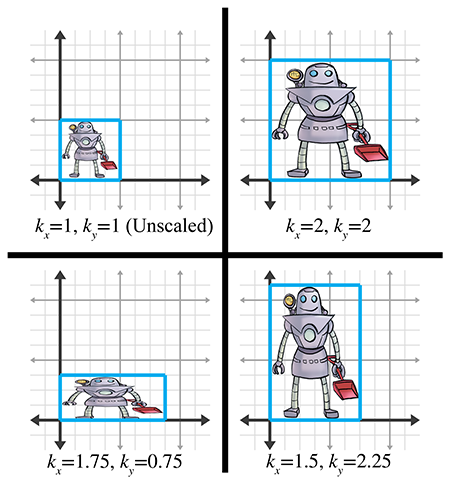
\includegraphics{05_scaling}
\caption{2D scaling}
\label{fig:2d-scaling}
\end{figure}

Scaling along the cardinal axes: \\
$$
\mathbf{S}(k_{x},k_{y}) =
\begin{bmatrix}
k_{x} & 0 \\
0 & k_{y} \\
\end{bmatrix}
$$

\subsubsection{Three dimensional}

Scaling along the cardinal axes: \\
$$
\mathbf{S}(k_{x},k_{y},k_{z}) = 
\begin{bmatrix}
k_{x} & 0 & 0 \\
0 & k_{y} & 0 \\
0 & 0 & k_{z}
\end{bmatrix}
$$

Scaling along an arbitrary vector: \\
$$
\mathbf{S}(\hat{\mathbf{n}},k) = \begin{bmatrix}
{1 + \left( k - 1 \right){n_{x}}^{2}} & {\left( k - 1 \right)n_{x}n_{y}} & {\left( k - 1 \right)n_{x}n_{z}} \\
{\left( k - 1 \right)n_{x}n_{y}} & {1 + \left( k - 1 \right){n_{y}}^{2}} & {\left( k - 1 \right)n_{y}n_{z}} \\
{\left( k - 1 \right)n_{x}n_{z}} & {\left( k - 1 \right)n_{y}n_{z}} & {1 + \left( k - 1 \right){n_{z}}^{2}} \\
\end{bmatrix}
$$

As an execise try scaling along the $x$-axis with a factor of $5$, that is $\mathbf{S}(
\begin{bmatrix}
1 & 0 & 0
\end{bmatrix},5)$. It will all make sense, or maybe not.

\subsection{Orthographic projection}

\begin{figure}[H]
\centering
    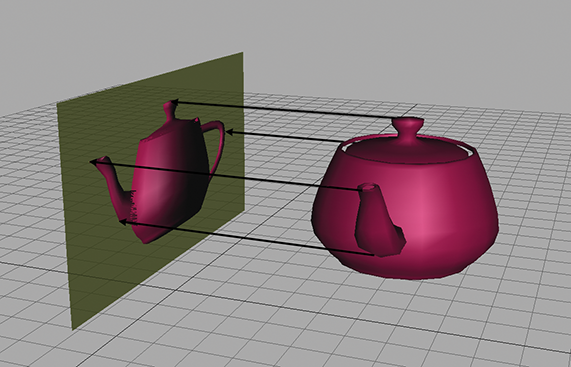
\includegraphics{05_projection}
\caption{2D projection}
\label{fig:2d-projection}
\end{figure}

The term \textit{projection} in general refers to any dimension reducing operation, so essentially we are going to discard some coordinate. This means we can scale some arbitrary vector by a scale of\dots $0$. No new derivations or matrices, simply use $\mathbf{S}(\hat{\mathbf{n}},0)$.

\subsection{Reflection}

\begin{figure}[H]
\centering
    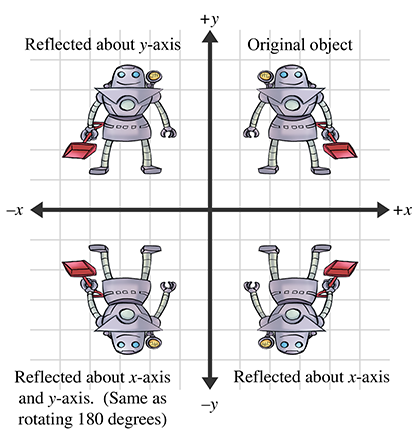
\includegraphics{05_reflection}
\caption{2D reflection}
\label{fig:2d-reflection}
\end{figure}

Reflection is flipping some axis once, that is, multiplying by $-1$. We once again use our scaling matrices, but this time with a value of $-1$. We can apply a reflection to any arbitrary vector as follows: $\mathbf{S}(\hat{\mathbf{n}},-1)$.

\subsection{Shearing}

\begin{figure}[H]
\centering
    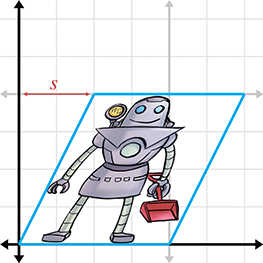
\includegraphics{05_shearing}
\caption{2D shearing}
\label{fig:2d-shearing}
\end{figure}

Shearing also known as skewing basically distorts the coordinate space as shown in the picture above. Check the book for the matrices as this transformation is seldom used, but you know, it's good to know it exists.


% Chapter 7 of the book
\newpage
\section{Polar Coordinate System}

As an alternative to the Cartesian coordinate system there exists the polar coordinate system. A (two dimensional) polar coordinate is described by a rotation and a radius. Like the Cartesian coordinate system we need to define a base grid with an origin and orientation, see figure \ref{fig:polar-coordinate-system}.

\begin{figure}[H]
\centering
    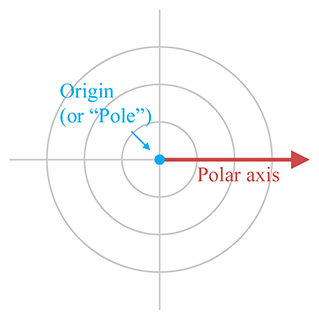
\includegraphics{07_polar_coordinate_system}
\caption{Polar coordinate system}
\label{fig:polar-coordinate-system}
\end{figure}

\subsection{Two dimensional polar coordinates}

The steps to take to find a polar coordinate $(r,\theta)$ are as follows: 

\begin{enumerate}
	\item Start at the origin facing the polar axis. Then rotate by the angle $\theta$, where a positive $\theta$ usually means counter clockwise rotation.
	\item Now move forward from the origin by a distance of $r$ units.
\end{enumerate}

\begin{figure}[H]
\centering
    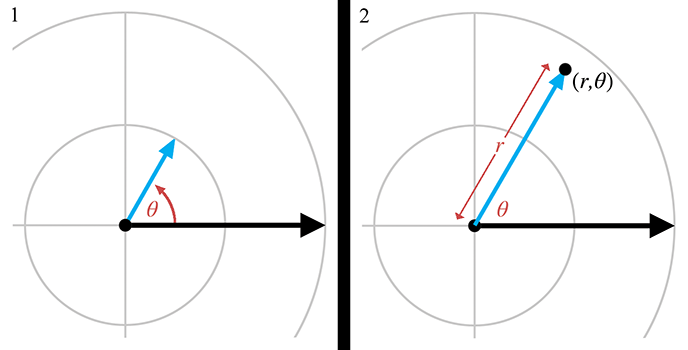
\includegraphics{07_2d_polar_coordinate}
\caption{Locating 2D polar coordinate}
\label{fig:locating-2d-polar-coordinate}
\end{figure}

\subsubsection{Canonical form}

As you might have noticed there exists aliasing of coordinates. For example, adding $2\pi$ to $\theta$ is aliases the original $\theta$. To avoid aliasing issues polar coordinates can be turned into canonical form:

\begin{itemize}
	\item $r \geq 0$, we don't measure distances "backwards".
	\item $-180^\circ < \theta \leq 180^\circ$, the angle is limited to half a revolution.
	\item $r=0 \implies \theta=0$, at the origin, set the angle to $0$.
\end{itemize}

An example C implementation can be found in the \path{code/} subdirectory with filename \path{07_canonical_2d_polar_coordinates.c}.

\subsubsection{Polar coordinate to Cartesian coordinate}

$$
\begin{array}{lr}
x=r\cos\theta; & y=r\sin\theta.
\end{array}
$$

\subsubsection{Cartesian coordinate to Polar coordinate}

$$
\begin{array}{lr}
r=\sqrt{x^2+y^2}; & \theta=\text{atan2}(y,x).
\end{array}
$$

Refer the book for a more depth explanation why we use $\text{atan2}$ rather than $\arctan$. An example C implementation can be found in the \path{code/} subdirectory with filename \path{07_2d_cartesian_to_polar.c}.

\subsubsection{atan2}

$\text{atan2}$ is a useful function to handle edge cases of $\arctan$. The following definition is roughly how it works in most computer languages. The exception being that $\text{atan2}$ is usually not defined for $(0,0)$, but for ease of use we do make this assumption. Furthermore, remember that the argument order is $y$ followed by $x$. Speaking from experience this is an easy mistake to make.

\begin{equation*}
	\text{atan2}(y,x) =
	\begin{cases}
		0, & x=0,y=0, \\
		+90^\circ, & x=0,y>0, \\
		-90^\circ, & x=0,y<0, \\
		\arctan(y/x), & x>0, \\
		\arctan(y/x)+180^\circ, & x<0,y\geq 0 \\
		\arctan(y/x)-180^\circ, & x<0,y<0
	\end{cases}
\end{equation*}

\subsection{Three dimensional polar coordinates}

The concept of polar coordinates can be extended to three dimensions in two distinct ways: cylindrical and spherical coordinates.

\subsection{Cylindrical coordinates}

The first type of the three dimensional polar coordinate is the cylindrical coordinate. The base of the cylinder is defined by a two dimensional polar coordinate, while the third coordinate is an axis like in Cartesian systems.

\begin{figure}[H]
\centering
    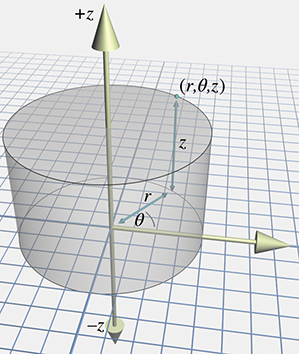
\includegraphics{07_cylindrical_coordinates}
\caption{Cylindrical coordinates}
\label{fig:cylindrical-coordinates}
\end{figure}

\subsubsection{Cylindrical coordinate to Cartesian coordinate}

$$
\begin{array}{lcr}
x=r\cos\theta; & y=r\sin\theta; & z=z.
\end{array}
$$

\subsubsection{Cartesian coordinate to Cylindrical coordinate}

$$
\begin{array}{lcr}
r=\sqrt{x^2+y^2}; & \theta=\text{atan2}(y,x); & z=z.
\end{array}
$$

\subsection{Spherical coordinates}

Unlike cylindrical coordinates, spherical coordinates are a bit more complex and require a bit more computation. A spherical coordinate is defined by two angles and a radius.

\begin{figure}[H]
\centering
    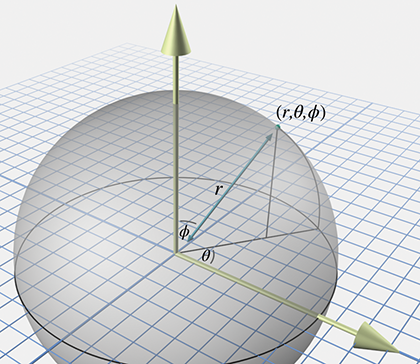
\includegraphics{07_spherical_coordinates}
\caption{Spherical coordinates}
\label{fig:spherical-coordinates}
\end{figure}

\subsubsection{Canonical Spherical coordinates}

Spherical coordinates has even more issues with regards to aliasing. So once again we define some common rules to avoid this. Where $\theta$ is replaced with the letter $h$ for heading, and $\phi$ replaced with the letter $p$ for pitch:

\begin{itemize}
	\item $r \geq 0$, we don't measure distances "backwards".
	\item $-180^\circ < h \leq 180^\circ$, the heading is limited to half a revolution.
	\item  $-90^\circ \leq p \leq 90^\circ$, pitch limits are straight up and down.
	\item $r=0 \implies h=p=0$, at the origin set the angles to $0$.
	\item $|p|=90^\circ \implies h=0$, when looking up or down set heading to $0$.
\end{itemize}

An example C implementation can be found in the \path{code/} subdirectory with filename \path{07_canonical_spherical_coordinates.c}.

\subsubsection{Canonical Spherical coordinate to Cartesian coordinate}

$$
\begin{array}{lcr}
x=r\cos p \sin h; & y=-r\sin p; & z=\cos p \cos h.
\end{array}
$$

\subsubsection{Cartesian coordinate to Canonical Spherical coordinate}

$$
\begin{array}{lcr}
r=\sqrt{x^2+y^2+z^2}; & h=\text{atan2}(x,z); & p=\arcsin(-y/r).
\end{array}
$$

An example C implementation can be found in the \path{code/} subdirectory with filename \path{07_3d_cartesian_to_spherical.c}.


% Chapter 8 of the book
\newpage
\section{Three dimensional rotations}

This chapter presents a short overview of three dimensional rotation methods, an overview of their usage and conversions between rotation methods.

Some important terms:

\begin{itemize}
	\item Direction: the vector where an object is pointing not taking into account the rotation around this axis.
	\item Orientation: direction with possible rotation around the direction. The difference between direction and orientation is a similar semantic issue as point and vector. For example, the direction of a airplane may be North, but the airplane might be twisted slightly. Describing both the direction and the twist is orientation. If you do not get, do not worry, or maybe do.
	\item Angular displacement: amount of rotation from some reference point. As you start to figure out; translation and rotation is always relative to some determined position. Everything in life is relative.
\end{itemize}

\subsection{Rotation matrices}

A rotation matrix describes the basis vectors of some coordinate space relative to another. Multiplying a vector by the matrix translates the matrix from object space to parent space. A vector in parent space can be transformed to object space by taking the inverse of the matrix. Note that this defintion of a matrix is a choice. We could have chosen to rotate from parent to object space by default too. The exact implementation details get a bit funky sometimes, but the concept is easy to understand. See section \ref{sec:rotation-matrices} for more details.

\subsection{Euler Angles}

Euler angles describe angular displacement as a sequence of three rotations around three mutually perpendicular axes. Common is to use the cardinal (object) axes in order of heading, pitch and finally bank. ($y$-axis, $x$-axis, and $z$-axis)

\subsubsection{Canonical Euler angles}

\begin{itemize}
	\item $-180^\circ < h \leq 180^\circ$
	\item $-90^\circ \leq h \leq 90^\circ$
	\item $-180^\circ < b \leq 180^\circ$
	\item $p=\pm 90^\circ \implies b=80^\circ$
\end{itemize}

\subsubsection{Wrap Pi}

A simple helper function to find the shortest arc between two rotations:

$$\text{wrapPi}(x)=x-360^\circ \lfloor \frac{x+180^\circ}{360^\circ} \rfloor$$

\noindent The result lies in the set $(-180^\circ,180^\circ]$.

\subsection{Axis-angle and exponential map}

Euler's rotation theorem (more or less) states that any angular displacement can be achieved by a single rotation around a carefully chosen axis. So, using this idea we and up with an angle $(\theta)$ and an axis $(\hat{\textbf{n}})$, which is exactly what the axis-angle format is.

A second approach is to multiply the angle with the axis. We will not lose any information, as the angle is a unit vector. Guess what, that is the definition of exponential map: $\textbf{e}=\theta\hat{\textbf{n}}$. The rotation can be found by taking the magnitude of the exponential map: $\theta=\|\textbf{e}\|$ from which follows that the axis equals $\hat{\textbf{n}}=\frac{\textbf{e}}{\|\textbf{e}\|}$.

Unlike quaternions, it is possible to capture arbitrary large rotations with these formats. Both $1080^\circ$ and $720^\circ$ end up in the same orientation; this distinction is not captured with quaternions. In certain use cases (e.g. angular velocity) this distinction is important, so it is good to know about the existence of these formats.

\subsection{Quaternions}

Quaternion is a rotation method that defines a three dimensional rotation with four numbers. By using four number quaternions avoid gimbal lock. In fact, quaternions are related to axis-angle representation. However, rather than storing the angle $(\theta)$ and axis $(\hat{\textbf{n}})$ as-is, the following notation is used:

$$
\textbf{q}=\begin{bmatrix}
	w & \textbf{v}
\end{bmatrix}=\begin{bmatrix}
	w & \begin{pmatrix}
		x & y & z
	\end{pmatrix}
\end{bmatrix}=\begin{bmatrix}
	\cos\frac{\theta}{2} & \sin\frac{\theta}{2}\hat{\textbf{n}}
\end{bmatrix}
$$

The notation is initially a bit weird, but it allows for a great property: unlike other rotation methods, it is possible to smoothly interpolate between two quaternion rotations with slerp (\textit{s}pherical \textit{l}inear int\textit{erp}olation). 

\subsubsection{Identity}

$$
\textbf{i}=\begin{bmatrix}
	1 & \textbf{0}
\end{bmatrix}=\begin{bmatrix}
	1 & \begin{pmatrix}
		0 & 0 & 0
	\end{pmatrix}
\end{bmatrix}
$$

\subsubsection{Negation}

$$-\textbf{q}=\begin{bmatrix}
	-w & -\textbf{v}
\end{bmatrix}=\begin{bmatrix}
	-w & \begin{pmatrix}
		-x & -y & -z
	\end{pmatrix}
\end{bmatrix}$$

The negation of a quaternion still descrbies the same angular displacement. Thus there technically are two identies, but the negated identity is rarely used.

\subsubsection{Magnitude}

$$\|\textbf{q}\|=\sqrt{w^2+\textbf{v}^2}=\sqrt{w^2+x^2+y^2+z^2}$$

For a rotation quaternion the magnitude equals $1$.

\subsubsection{Conjugate}

$$\textbf{q}^*=\begin{bmatrix}
	w & \textbf{v}
\end{bmatrix}^*=\begin{bmatrix}
	w & -\textbf{v}
\end{bmatrix}=\begin{bmatrix}
	w & \begin{pmatrix}
		-x & -y & -z
	\end{pmatrix}
\end{bmatrix}$$

The conjugate is simply negating the vector part of the quaternion. The term conjugate is inherited from complex numbers.

\subsubsection{Inverse}

$$\textbf{q}^{-1}=\frac{\textbf{q}^*}{\|\textbf{q}\|}$$

For rotation quaternions $\textbf{q}^{-1}=\textbf{q}^*$, because the magnitude is always $1$. Furthermore, $\textbf{q}\textbf{q}^{-1}=\textbf{i}$.

\subsubsection{Multiplication}

$$
\textbf{q}_1\textbf{q}_2=\begin{bmatrix}
	w_1 & \textbf{v}_1
\end{bmatrix}\begin{bmatrix}
	w_2 & \textbf{v}_2
\end{bmatrix}=\begin{bmatrix}
	w_1w_2-\textbf{v}_1\cdot\textbf{v}_2 \\
	\begin{pmatrix}
		w_1\textbf{v}_2 + w_2\textbf{v}_1 + \textbf{v}_1\times\textbf{v}_2
	\end{pmatrix}
\end{bmatrix}
=\begin{bmatrix}
	w_1w_2-x_1x_2-y_1y_2-z_1z_2 \\
	\begin{pmatrix}
		w_1x_2 + x_1w_2 + y_1z_2 - z_1y_2 \\
		w_1y_2 + y_1w_2 + z_1x_2 - x_1z_2 \\
		w_1z_2 + z_1w_2 + x_1y_2 - y_1x_2
	\end{pmatrix}
\end{bmatrix}
$$

Multiplication of two quaternions adds their rotations together; it is also known as the Hamilton product. Multiplication guarantees a unit quaternion, because $\|\textbf{q}_1\textbf{q}_2\|=\|\textbf{q}_1\|\|\textbf{q}_2\|$. Quaternions are not commutative $\textbf{q}_1\textbf{q}_2\neq\textbf{q}_2\textbf{q}_1$. Moreover, $(\textbf{ab})^{-1}=\textbf{b}^{-1}\textbf{a}^{-1}$. Lastly, rotation some point $(\textbf{p})$ by a quaternion can be done with the formula: $\textbf{qp}\textbf{q}^{-1}$.

\subsubsection{Difference}

The difference $(\textbf{d})$ from quaternion $\textbf{a}$ to $\textbf{b}$:

$$
\textbf{d}=\textbf{b}\textbf{a}^{-1}
$$

\subsubsection{Dot product}

$$
\textbf{q}_1\cdot\textbf{q}_2=\begin{bmatrix}
	w_1 & \textbf{v}_1
\end{bmatrix}\cdot\begin{bmatrix}
	w_2 & \textbf{v}_2
\end{bmatrix}=
w_1w_2+\textbf{v}_1\cdot\textbf{v}_2
$$

The quaternion dot product is used in slerp. Remember that the vector dot product gives the cosine of the angle between two vectors, whereas the quaternion dot product gives the cosine of half the angle needed to go from one quaternion to the other.

\subsubsection{Log and Exp}

$$\log\textbf{q}=\log\begin{bmatrix}
\cos\frac{\theta}{2} & \hat{\textbf{n}}\sin\frac{\theta}{2}\end{bmatrix}\equiv
\begin{bmatrix}0 & \frac{\theta}{2}\hat{\textbf{n}}\end{bmatrix}$$

$$\exp\textbf{q}=\exp\begin{bmatrix}0 & \frac{\theta}{2}\hat{\textbf{n}}\end{bmatrix}=
\begin{bmatrix}\cos\frac{\theta}{2} & \hat{\textbf{n}}\sin\frac{\theta}{2}\end{bmatrix}
$$

$$\exp(\log\textbf{q})=\textbf{q}$$

\subsubsection{Scalar multiplication}

$$k\textbf{q}=k\begin{bmatrix}w & \textbf{v}\end{bmatrix}=
\begin{bmatrix}kw & k\textbf{v}\end{bmatrix}$$

\subsubsection{Exponentiation}

$$\textbf{q}^t=\exp(t\log\textbf{q})$$

Note how exponentiation reuses the definitions of the previous sections. Quaternion exponentiation has a similar use like scalar exponentiation. For scalars we know that $1$: $a^0=1$ where $a \neq 0$ and $a^1=a$. The same works for quaternions with on caveat. If a quaternion describes a rotation of $30^\circ$, then $\textbf{q}^8$ will \textbf{not} describe a rotation of $240^\circ$, but $120^\circ$ instead! A quaternion always represents the shortest arc. If such behavior is required, one must use axis-angle or an exponential map.

A way to look at the above equation is that $\log$ converts the quaternion to exponential map format (with a factor of 2), the angle then gets multiplied by $t$, and finally $\exp$ calculations the new $w$ and $\textbf{v}$ from the exponential vector.

A practical implementation can be found in the code snippet \path{08_quaternion_exponentiation.c}.

\subsubsection{Slerp}

Spherical linear interpolation, slerp for short, allows for smooth interpolation between two rotations. Recall, linear interpolation between two scalars:

\begin{align*}
\Delta a &= a_1 - a_0 \\
\text{lerp}(a_0, a_1, t) &= a_0 + t \Delta a
\end{align*}

Essentially, we want to achieve the same thing for quaternions. The steps to take is to compute the difference, take some fraction of this difference, and add this fraction to the original orientation.

\begin{enumerate}
	\item Computing the difference can be done with the formula $\Delta \textbf{q} = \textbf{q}_1\textbf{q}_0^{-1}$ as described in a previous section.
	\item A fraction can be calculated using exponentiation: $(\Delta \textbf{q})^t$.
	\item The original value and the computed fraction can be composed using multiplication: $(\Delta \textbf{q})^t\textbf{q}_0$.
\end{enumerate}

\noindent Putting it all together:

$$\text{slerp}(\textbf{q}_1,\textbf{q}_2,t)=(\textbf{q}_1\textbf{q}_0^{-1})^t\textbf{q}_0$$

So, we figured out how slerp works: hurray! Well\dots, we figured out the theory. An implementation can be found in the code snippet \path{08_slerp.c}, which differs a bit from the equations above. It makes use of the fact that quaternions are of unit length and live on the same four-dimensional hypersphere, hence \textit{spherical} linear interpolation. The exact math related to the code can be found in the book (in case you want to write your own math library).


% Chapter 9 of the book
\newpage
\section{Geometric primitives}

\subsection{Lines and rays}

Types of lines:
\begin{enumerate}
	\item Infinite line in both directions.
	\item Line segment: finite line between two points.
	\item Ray Some origin and infinite extension in some direction. In computer graphics we often make use of a finite ray however.
\end{enumerate}

\subsection{Spheres and circles}

Some important functions with regards to spheres and circles.

\begin{itemize}
	\item Implicit definition of 2D circle: $(x-c_x)^2 + (y-c_y)^2=r^2$
	\item Implicit definition of 3D sphere: $(x-c_x)^2 + (y-c_y)^2+ (z-c_z)^2=r^2$
	\item Common formulas:
	\begin{align*}
		D &= 2r &(\text{diameter}) \\
		C &= 2\pi{}r = \pi{}D &(\text{circumference}) \\
		A &= \pi{}r^2 &(\text{area of circle}) \\
		S &= 4\pi{}r^2 &(\text{surface area of sphere}) \\
		V &= \frac{4}{3}\pi{}r^3 &(\text{volume of sphere})
	\end{align*}
\end{itemize}

\subsection{Bounding boxes}

Types of bounding boxes:
\begin{enumerate}
	\item AABB: the box is aligned to the world's axes.
	\begin{itemize}
		\item All points are defined by:
		\begin{align*}
			x_{min} &\leq x \leq x_{max} \\ 
			y_{min} &\leq y \leq y_{max} \\
			z_{min} &\leq z \leq z_{max}
		\end{align*}
		\item $p_{min}=\begin{bmatrix}
			x_{min} & y_{min} & z_{min}
		\end{bmatrix}$
		\item $p_{max}=\begin{bmatrix}
			x_{max} & y_{max} & z_{max}
		\end{bmatrix}$
		\item $center= (p_{min} + p_{max}) / 2$
		\item $size = p_{max} - p_{min}$
		\item $radius = size / 2$
	\end{itemize}
	\item OBB: the box is aligned in object space.
	\item Spheres can also be used as bounding box (uh sphere). They are easy to use for intersection, but often poorly wrap around objects.
\end{enumerate}

\subsection{Planes}

\begin{itemize}
	\item Implicit definition of a plane: $\textbf{p} \cdot \hat{\textbf{n}}=d$. Where $\textbf{n}$ is the vector perpendicular to the plane and $d$ the distance from the origin.
	\item The plane normal ($\hat{\textbf{n}}$) can be calculated for any three noncollinear points with the following formulas:
	\begin{enumerate}
		\item $\textbf{e}_3 = \textbf{p}_2 - \textbf{p}_1$,
		\item $\textbf{e}_1 = \textbf{p}_3 - \textbf{p}_2$,
		\item $\hat{\textbf{n}}=\frac{\textbf{e}_3 \times \textbf{e}_1}{\| \textbf{e}_3 \times \textbf{e}_1 \|}$.
		\item $d=\hat{\textbf{n}} \cdot \textbf{p}_1$
	\end{enumerate}
	\item Distance of some point, $\textbf{q}$, to the plane can be computed with the formula: $distance = \textbf{q} \cdot \hat{\textbf{n}} - d$.
	\item See exercise 5 of chapter 9 for an interesting algorithm to find the best fit plane for a set of points.
\end{itemize}

\subsection{Triangles}

\subsubsection{Notation}

In a left-handed system the vertices of triangles are defined clockwise, while in right-handed system the vertices are defined counter-clockwise.

\begin{figure}[H]
\centering
    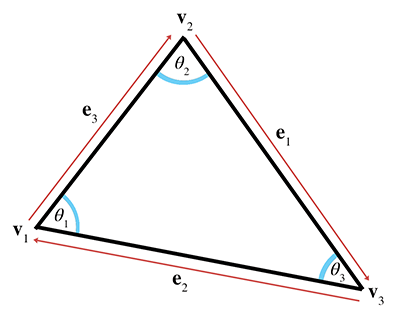
\includegraphics{09_triangle_notation}
\caption{Triangle notation}
\label{fig:triangle-notation}
\end{figure}

Formulas for all edges and lengths:

\begin{align*}
\textbf{e}_1 &= \textbf{v}_3 - \textbf{v}_2, & \textbf{e}_2 &= \textbf{v}_1 - \textbf{v}_3, & \textbf{e}_3 &= \textbf{v}_2 - \textbf{v}_1, \\
l_1& = \|\textbf{e}_1\|, & l_2 &= \|\textbf{e}_2\|, & l_3 &= \|\textbf{e}_3\|, \\
\end{align*}

The perimeter is defined by the sum of lengths: $p = l_1 + l_2 + l_3$.

Also, remember the sine and cosine laws from section \ref{sin_cos_laws}.

\subsubsection{Area}

The triangle area can be calculated with $\frac{\text{base}\cdot{}\text{height}}{2}$. A second approach is using the cross product: 

$$A=\frac{\| \textbf{e}_1 \times \textbf{e}_2 \|}{2}$$

\noindent{} Personally, I like this approach best. It works for 3D and 2D.

\subsubsection{Barycentric coordinates}

A barycentric coordinate is the weighted average of the three vertices of a triangle. $(b_1, b_2, b_3) \equiv (b_1\textbf{v}_1+b_2\textbf{v}_2+b_3\textbf{v}_3)$. The requirement is that $b_1+b_2+b_3=1$.

\begin{figure}[H]
\centering
    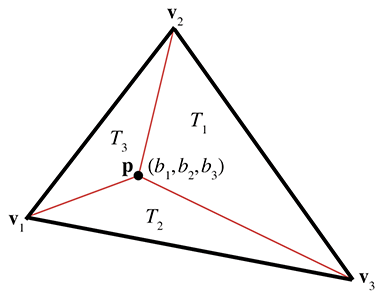
\includegraphics{09_barycentric_coordinates}
\caption{Barycentric coordinates}
\label{fig:barycentric-coordinates}
\end{figure}

Refer the book and the \path{exercise04.cpp} in \path{chapter09} for algorithms to compute barycentric coordinates.

\subsubsection{Center of gravity}

\begin{figure}[H]
\centering
    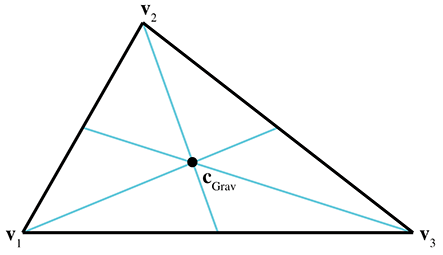
\includegraphics{09_center_of_gravity}
\caption{Center of gravity}
\label{fig:center-of-gravity}
\end{figure}

The center of gravity can be computed as follows:

$$\textbf{c}_{\text{Gravity}}= \frac{\textbf{v}_1+\textbf{v}_2+\textbf{v}_3}{3}$$

\noindent Barycentric notation: 

$$\left( \frac{1}{3}, \frac{1}{3}, \frac{1}{3} \right)$$

\subsubsection{Incenter}

\begin{figure}[H]
\centering
    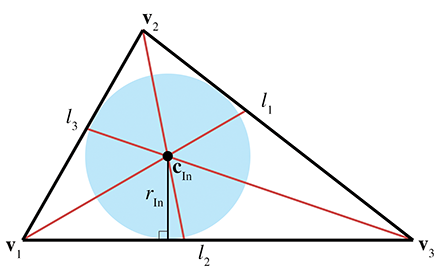
\includegraphics{09_incenter}
\caption{Incenter}
\label{fig:incenter}
\end{figure}

The incenter is computed by:

$$\textbf{c}_{\text{In}} = \frac{l_1\textbf{v}_1 + l_2\textbf{v}_2 + l_3\textbf{v}_3}{p}$$

\noindent Barycentric notation:

$$\left(\frac{l_1}{p}, \frac{l_2}{p}, \frac{l_3}{p}\right)$$

\noindent Radius of incenter:

$$r_{\text{In}} = \frac{A}{p}$$

\subsubsection{Circumcenter}

\begin{figure}[H]
\centering
    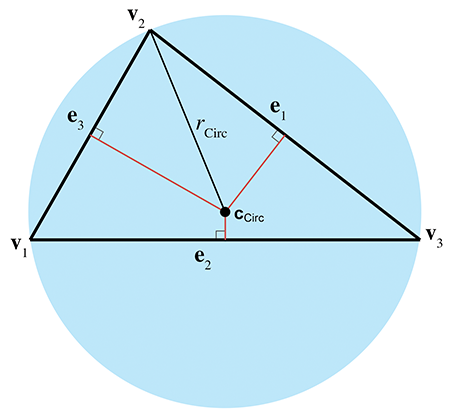
\includegraphics{09_circumcenter}
\caption{Circumcenter}
\label{fig:circumcenter}
\end{figure}

The circumcenter is the point the is equidistant from all vertices. It solves the problem of finding a circle that passes through three points. The computation is a bit length, so just refer the book whenever you need this.

\subsection{Polygons}

Polygons are quite hard to define, but basically it are shapes made up of vertices and edges. Some important terms to know about:

\begin{itemize}
	\item \textit{Simple} polygon: a polygon without any holes.
	\item \textit{Complex} polygon: a polygon that may have holes.
	
\begin{figure}[H]
\centering
    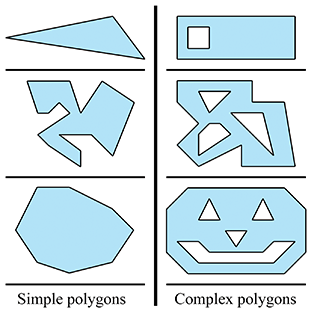
\includegraphics{09_simple_complex}
\caption{Simple and complex polygons}
\label{fig:simple-complex-polygons}
\end{figure}

	\item \textit{Convex} polygon: a polygon without dents, all edges between all vertices are contained in the polygon.
	\item \textit{Concave} polygon: a polygon with some dent, at least one edge between any pair of vertices is outside the polygon.
	
\begin{figure}[H]
\centering
    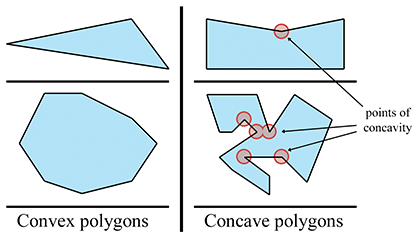
\includegraphics{09_convex_concave}
\caption{Convex and concave polygons}
\label{fig:convex-concave-polygons}
\end{figure}	
	
	\item Polygons can be divided into triangles. For complex polygons this is quite tricky, but for any convex it is quite easy. It can be done by a method called \textit{fanning}, which basically adds extra edges to subdivide the polygon into triangles.
\begin{figure}[H]
\centering
    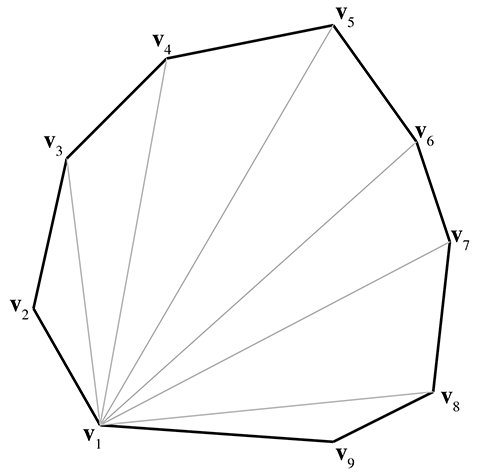
\includegraphics{09_fanning}
\caption{Fanning of convex polygon}
\label{fig:convex-fanning}
\end{figure}

\end{itemize}


% Chapter 11 and 12 of the book
\newpage
\section{Mechanics}

\subsection{Overview of common physical quantities}

\begin{figure}[H]
\centering
    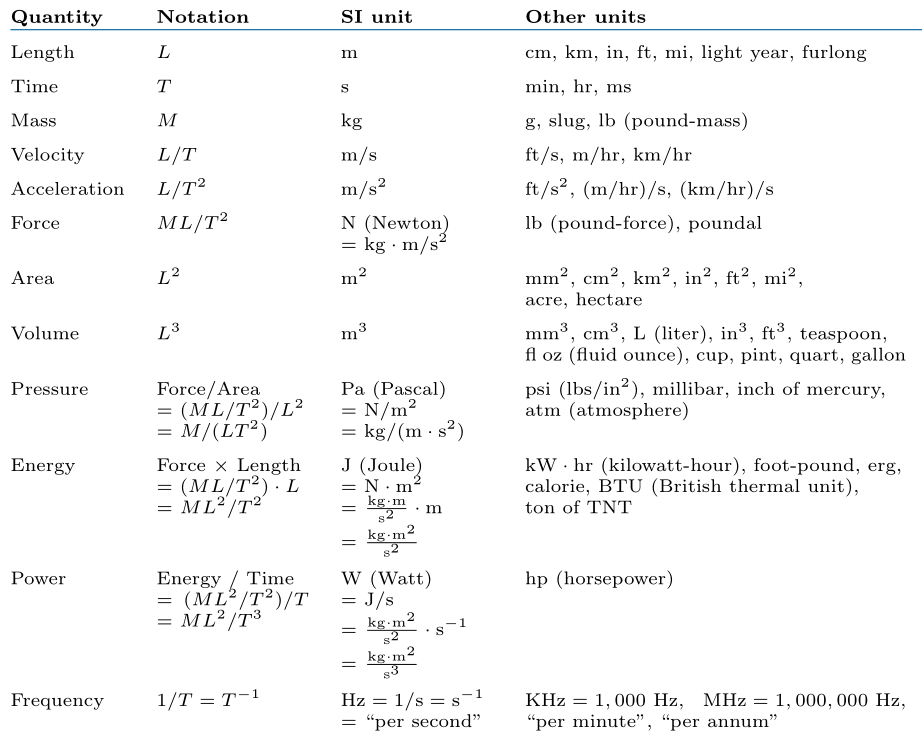
\includegraphics[width=\textwidth]{11_physical_quantities}
\caption{Selected physicial quantities}
\label{fig:physical-quantities}
\end{figure}

Velocity is a vector of displacement, while speed is a scalar of the rate at which an object is moving. The derivative measures the rate of change, since velocity measures the rate of change of position with respect to time, the velocity function is the derivative of the position function.

\subsection{Taylor series}

\begin{itemize}
	\item $\sin x = x - \frac{x^3}{3!} + \frac{x^5}{5!} - \frac{x^7}{7!} + \frac{x^9}{9!} + \dots$
	\item $\cos x = 1 - \frac{x^2}{2!} + \frac{x^4}{4!} - \frac{x^6}{6!} + \frac{x^8}{8!} + \dots$
	\item $e^x = 1 + x + \frac{x^2}{2!} + \frac{x^3}{3!} + \frac{x^4}{4!} + \dots$
\end{itemize}

Taking the derivatives and integrals from these series makes the derivatives definitions very obvious.

\subsection{Derivative definition}

$$\frac{dy}{dx}=\lim_{h \to 0} \frac{y(x+h)-y(x)}{h}$$

\subsection{Common derivatives}

\begin{itemize}
	\item $\frac{d}{dx}\sin x = \cos x$
	\item $\frac{d}{dx}\cos x = -\sin x$
	\item $\frac{d}{dx}e^x = e^x$
\end{itemize}

\end{document}
